\documentclass{Math_Note}

\title{The Stardew Sky of Prime Numbers}
\author{Buce-Ithon}
\newdateformat{mydate}{\twodigit{\THEDAY}{ }\shortmonthname[\THEMONTH], \THEYEAR}
\date{\today}

\begin{document}

%Title page
\maketitle

%Content
\newpage
\tableofcontents
\newpage

%Beginning
\section{Introduction}

\begin{mdframed}
    \textit{From Wikipedia:}\\
    The Ulam spiral or prime spiral is a graphical depiction of the set of prime numbers, devised by mathematician Stanisław Ulam in 1963 
    and popularized in Martin Gardner's Mathematical Games column in Scientific American a short time later. It is constructed by writing 
    the positive integers in a square spiral and specially marking the prime numbers.
\end{mdframed}

There are many beautiful laws in nature. The integers are stars of the reals, and the prime numbers are stars of the integers. In this article, 
we'll explore the distribution or to say "stardew sky" of prime numbers.

%Bady
\section{The Stardew sky of Prime Numbers}

The Ulam spiral is constructed by writing the positive integers in a spiral arrangement on a square lattice:

\begin{figure}[H]
    \centering
    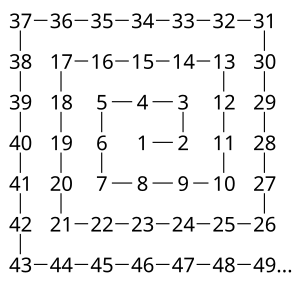
\includegraphics[scale=0.32]{"./Figures/Ulam_spiral_1.png"}
    \caption{Spiral of Positive Integers}
\end{figure}

then we mark the prime numbers in the spiral:

\begin{figure}[H]
    \centering
    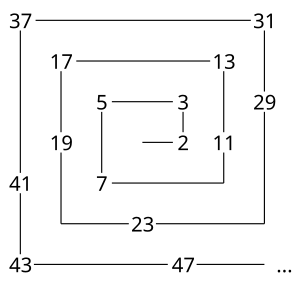
\includegraphics[scale=0.32]{"./Figures/Ulam_spiral_2.png"}
    \caption{Ulam Spiral of Positive Prime Numbers}
\end{figure}

We could find that mostly all the corner of the spiral are prime numbers. This is a very interesting phenomenon.

\textbf{Extension:} Of course, we can also use triangular spiral or even curves to represent the prime numbers.(Figures are waiting for you to explore) 

\section{Questions}

\textbf{Q1.} If we use other current situations to construct spirals, what will be the rules for the distribution of prime numbers?

\textbf{Q2.} If we draw a circle with radius $r$ around the origin, what is the density of prime numbers inside the circle?

\end{document}